%-------------------------
% CHAPTER 11: Conclusions
%-------------------------

\chapter{Conclusions} \label{chapter11}

After almost six months of the development of a full stack project and after the whole report of the \thesis, there are some conclusions.

\section{Results}

Sadly, results are not the expected, maybe in the beginning the idea was too optimistic thinking that it would be easy to make assumptions when comparing available flights and user searches.
\\\\
From the beginning it was known that one value was for available flights without counting seats of the aircraft or actual \textbf{available seats}, and the other one were searches. Here is an example of why the comparison is not as good as expected:

\begin{figure}[H]
\centering
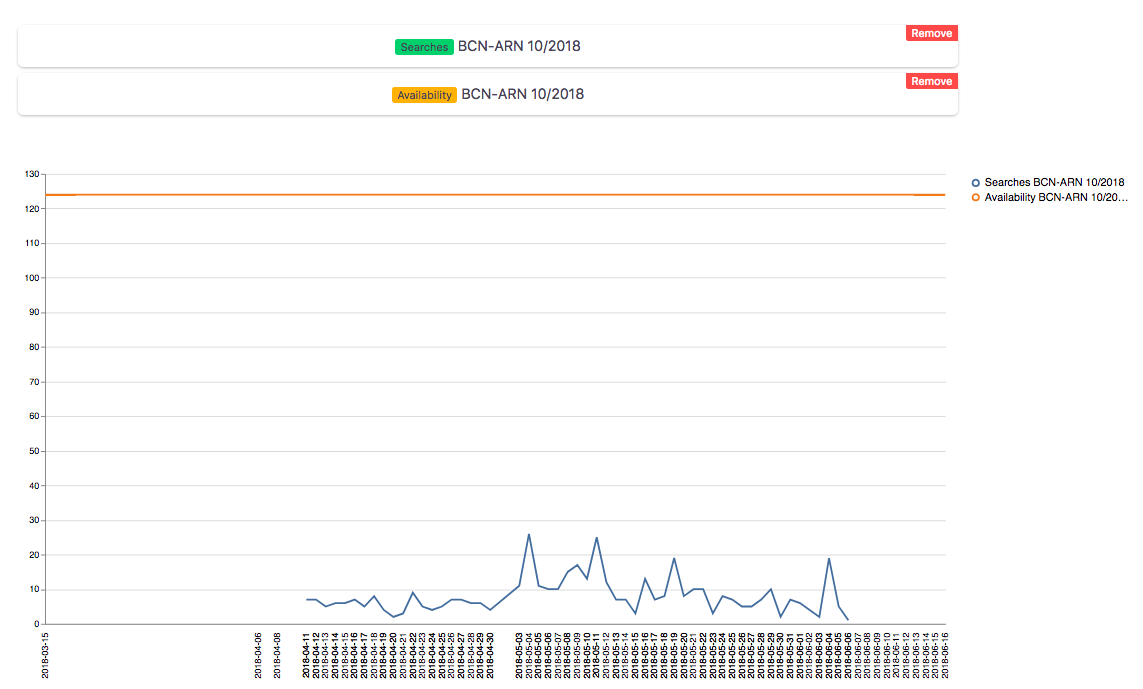
\includegraphics[scale=0.3]{resources/experiment03.png}
\caption{Comparison from Barcelona to Stockholm, October 2018}
\end{figure}

Sometimes, data is not what looks like.
\\\\
Luckily, same source comparisons can give relevant results, see \nameref{exp1} on page \pageref{exp1} and \nameref{exp2} on page \pageref{exp2}.
\\\\
Apart from that issue, all functional and non-functional requirements are fully satisfied. \textbf{The project is completed and works fine}.

\section{Development}

The most valuable thing of this project is the knowledge earned during the making of it. Not only as a programmer, but as a Software Engineer.

\subsubsection*{Inception}

In the beginning looked impossible to find stakeholders and define the project. Being new in the company, was kind of intimidating start talking to product owners. Thanks to my Squad Lead I met them and defined something promising, he set some meetings with product owners he already knew and I end up doing \textbf{elevator pitch}es to them.
\\\\
Now that I am in the end of the project and I know more people and how things work inside of \company, it would be much easier for me to do that process. I would not be afraid of talking to some Product Owners. I can say that \textbf{I learned how to sell a software idea} to anyone, in this case inside the same company.

\subsubsection*{Ping pong}

When specifying and developing the \thesis, if I had some question, I have done \textbf{\textit{ping pong}} between a lot of people. The process is usually the same: You ask something to someone you think they know the answer, but they do not. If you are lucky, they send you to someone that actually knows the answer. But what usually happens next is that they send you to someone they think they know the answer, but they do not neither. The process repeats and repeats until you find the answer.

\subsubsection*{Architecture}

When designing the architecture, I learned a lot. There has been a lot of analysis to different technologies, a lot of alternatives has been studied and discarded, finding a final solution.

\subsubsection*{Methodology}

The agile methodology has been great, but there has been some big blockers that was caused because of the methodology of the company: It took one month to get access to Athena, the ticket I opened to get access to it took a lot of time to be validated and processed.
\\\\
Sometimes it is good to work in a big company because you have a lot of resources that in a start up you cannot get, but for cases like these, you have less \textit{freedom}.

\section{Final conclusion}

It has been great to work in a project of these dimensions. From the beginning until the end.
\\\\
I have learned a lot of great development practices, used different technologies and combined them, I have taken risks always into account and applied different strategies for them and delivered a satisfactory product. I brought something good for Skyscanner.
\\\\
\begin{center}
\textit{The end.}
\end{center}

